\chapter{Introduction aux Malwares et Antivirus}
\section{Introduction}
De nos jours les entreprises et les particuliers sont de plus en plus interconnectés via Internet pour des raisons diverses, par exemple : l'accès à des services bancaires, vente en ligne, échanges de données ...\\
Cette évolution offre évidement beaucoup d'avantages mais elle s'accompagne également du risque inquiétant d'attaques contre les systèmes informatiques. Ces attaques peuvent se présenter sous plusieurs formes comme : le vol de données confidentielles, l'accès illégal au compte utilisateur, la diffusion de codes malicieux,...\\
Compte tenu des conséquences de ces types de menace, l'installation des systèmes de sécurité est devenue indispensable face aux nouvelles techniques d'attaques qui reposent sur des méthodes de plus en plus complexes et sophistiquées.
\section{Terminologie}
\subsection{La sécurité du système d'information}
Ensemble de mesures de sécurité physique, logique, administrative et de mesures d'urgence, mises en place dans une organisation, en vue d'assurer :
\begin{itemize}
\item la confidentialité et l'intégrité des données de son système d'information
\item la protection de ses biens informatiques
\item la continuité de service~\cite{sec}.
\end{itemize}
\subsection{Vulnérabilités}
Ce sont des vulnérabilités de sécurité dans un ou plusieurs systèmes permettant à un intrus de placer un système informatique dans un état qui accroît le risque de comportement indésirable du système et qui est contraire aux souhaits du responsable du système~\cite{vuln}. Ces vulnérabilités peuvent être ou non exploitable.\\
Exemples de vulnérabilités :
\begin{itemize}
\item utilisation des mots de passe non robustes
\item présence de comptes non protégés par mot de passe
\item vulnérabiltiés logicielles (débordements de tampon, injections SQL, ...)
\item faiblesses cryptographiques.
\end{itemize}
\subsection{Menaces}
Une menace est un événement ou une circonstance ayant le potentiel d'endommager un système informatique en le détruisant, le divulguant, modifiant ses données, et/ou en faisant un déni de services~\cite{men}.\\
les menaces peuvent être accidentelles comme:
\begin{itemize}
\item panne disque
\item chute de tension
\item échange des disquettes infectée
\end{itemize}
ou bien intentionnelles comme:
\begin{itemize}
\item le vol
\item l'écoute
\item la fouille.
\end{itemize}
\subsection{Attaques}
Les attaques sont les moyens d'exploiter une vulnérabilité afin d'obtenir un accès non autorisé aux services, ressources, ou informations d'un système d'informations. C'est aussi la tentative de compromettre l'intégrité, la disponibilité, ou la confidentialité d'un système informatique~\cite{men}.
\subsubsection{Les attaques d'accès}
parmis ces attaques nous trouvons:
\begin{itemize}
\item \textbf{Ingénierie sociale :} l'attaquant établit des relations avec le personnel pour obtenir des
informations sur les mots de passe, La topologie du réseau,...
\item \textbf{Portes dérobées (backdoors) :} injecter un code dans la cible pour l'exploiter plus tard
\item \textbf{Sniffing :} l'attaquant se met à l'écoute sur le réseau pour obtenir des informations.
\end{itemize}
\subsubsection{Les attaques de modification}
Ces attaques visent l'intégrité des informations (modification, rejeu, ... ), tel que les virus, les vers et les trojans.
\subsubsection{Les attaques par saturation}
\begin{itemize}
\item \textbf{Le flooding : }envoyer à une machine de nombreux paquets d'une forme spécialement conçue. La machine cible ne pourra pas traiter tous les paquets et finira par se déconnecter du réseau
\item \textbf{Le smurf : }cela consiste à envoyer une trame ICMP à une adresse IP de Broadcast réseau. Le but est de coupler cette trame à une adresse IP source correspondante à celle de la cible. Et grâce à cela, le flux de réponse en destination de la cible sera multiplié
\item \textbf{Le débordement de tampon : }une attaque par débordement de tampon consiste à exploiter une vulnérabilité  applicative sur la machine cible afin d'y exécuter un code arbitraire qui la compromettra. Pour cela, on fait planter le programme en provoquant un dépassement de capacité du tampon par injection de données, le surplus de données est mis dans les tampons adjacents, ce qui écrasera l'adresse de retour de la fonction en cours d'exécution. On peut donc choisir les prochaines instructions qui seront exécutées par le processeur.
\end{itemize}
\subsubsection{Les attaques de répudiation}
\begin{itemize}
\item \textbf{IP spoofing :}L'IP spoofing est une technique qui consiste à masquer l'identité de l'attaquant en changeant l'adresse IP source. On peut facilement coupler cette technique à d’autres techniques d’attaques ne nécessitant pas de réponse, comme le ping flood, UDP flood, SYN flood, l’attaque ICMP redirect, et bien d’autres.
\end{itemize}
\subsection{Faux positif et faux négatif}


Un faux positif est une erreur de jugement d'un programme de détection, qui va réagir et renvoyer une alerte alors qu'il n'y a pas lieu de le faire. Pour un antivirus, cela se produit lorsque le programme scanne un fichier sain et le déclare infecté (positif pour son test) alors qu'il ne l'est pas.\\


Un faux négatif est l'absence de détection d'une vulnérabilité ou le non déclenchement d'une alerte d'intrusion.

\section{Les Malwares}

\subsection{Définition}
Les travaux de Cohen ~\cite{coh} en 1986 et Adleman ~\cite{adl} en 1988 constituent les fondements de la virologie. Un virus, au sens de Cohen, peut être formalisé par un mot sur le ruban (zone mémoire) d'une machine de Turing, qui se duplique ou se modifie sur ce même ruban lorsqu'il est activé. La notion de réplication automatique est une caractéristique primordiale du virus. Adleman propose une notion plus générale d'infection informatique. La réplication n'entre pas dans sa définition qui est alors élargie à tout programme nuisible pour la machine ou l'utilisateur. \\


Dans son livre, Filiol ~\cite{anti} propose la définition suivante pour une infection informatique ou malware:\\


Définition : \textit{
Programme simple ou auto-reproducteur, à caractère offensif, s'installant dans 
un système d'informations, à l'insu du ou des utilisateurs, en vue de porter atteinte
à la confidentialité, l'intégrité, ou la disponibilité de ce système, ou susceptible 
d'incriminer à tort son possesseur ou l'utilisateur dans la réalisation d'un crime 
ou d'un délit.}\\

\subsection{Catégories des malwares}
Voici les principaux types de programmes malveillants :

\subsubsection{Les Virus}
Un virus est un logiciel malveillant, généralement de petite taille, qui se transmet par les réseaux ou les supports d'information amovibles, s'implante au sein des programmes en les parasitant, se duplique à l'insu des utilisateurs et produit ses effets dommageables quand le programme infecté est exécuté ou quand survient un évènement donné~\cite{virus}.\\
On distingue :
\begin{itemize}


\item \textbf{ le virus de boot :} il est chargé en mémoire au démarrage et prend le contrôle de l'ordinateur
\item \textbf{ le virus d'application :} il infecte un programme exécutable et se déclenche à l'exécution de celui-ci
\item \textbf{ le macro virus :} il infecte les documents bureautiques en utilisant leur langage de programmation.
\end{itemize}
\subsubsection{Les vers (worms)}
Un ver informatique est un logiciel malveillant qui se reproduit sur des ordinateurs à l'aide
d'un réseau informatique comme l'Internet ou tout autre support permettant sa propagation.\\
Un ver, contrairement à un virus informatique, n'a pas besoin d'un programme hôte pour se
reproduire. Il exploite les différentes ressources afin d'assurer sa reproduction. La définition d'un ver s'arrête à la manière dont il se propage de machine en machine, mais le véritable but de tels programmes peut aller au delà du simple fait de se reproduire : espionner, offrir un point d'accès caché (porte dérobée), détruire des données, faire des dégâts, envoi de multiples requêtes vers un site Internet dans le but de le saturer, etc. Les effets secondaires peuvent être aussi un ralentissement de la machine infectée, ralentissement du réseau, plantage des services ou du système, etc ~\cite{ver}.\\

Des vers écrits sous forme de script peuvent être intégrés dans un courriel ou sur une page
HTML sur Internet. Ils sont activés par les actions de l'utilisateur qui croit accéder à des
informations lui étant destinées.\\
Un ver peut tout aussi bien être programmé en C, C++, Delphi, assembleur, etc. Il utilise la
plupart du temps des bugs de logiciels pour se propager.


\subsubsection{Cheval de Troie (trojan)}
Un cheval de Troie est un programme installé par des pirates informatiques de manière invisible et frauduleuse. Il peut-être intégré dans la pièce-jointe d’un courriel via un lien Internet piégé, par échange de clés USB ou par le téléchargement de logiciel. L’objectif est de pouvoir exécuter des actions à l'insu de l'utilisateur (récupération, détournement, diffusion ou destruction des données), et /ou pour prendre à distance, le contrôle de l'ordinateur. Contrairement aux vers et virus, les chevaux de Troie ne se reproduisent pas. \\

Les chevaux de Troie servent très fréquemment à introduire une porte dérobée sur un
ordinateur. L'action nuisible à l'utilisateur est alors le fait qu'un pirate informatique peut à tout moment prendre à distance (par Internet) le contrôle de l'ordinateur~\cite{troj}.
\subsubsection{Logiciel espion (spyware)}
Les spywares, ou logiciels espions, permettent de voler des données utilisateur : mots de passe, documents, clés d'enregistrement de logiciels, adresses électroniques, etc. Les données sont recherchées sur les supports de données ou sont filtrées à partir du trafic réseau. Les données saisies au niveau des formulaires Web (des banques en ligne, notamment) sont également collectées. Dans le pire des cas, les pirates ont alors accès à tous les comptes de messagerie, forums et boutiques en ligne utilisés par la victime. Les spywares sont généralement très utilisés par les cybercriminels.
\subsubsection{Les portes dérobées (backdoor)}
Une porte dérobée peut être introduite soit par le développeur du logiciel, soit par un tiers,
typiquement un pirate informatique. La personne connaissant la porte dérobée peut l'utiliser pour surveiller les activités du logiciel, voire en prendre le contrôle (par contournement de
l'authentification)~\cite{mal}.\\
Parmi les motivations amenant les développeurs de logiciel à créer des portes dérobées :
\begin{itemize}
\item l'intérêt pratique d'un accès facile et toujours ouvert au logiciel pour pouvoir mener efficacement les actions de maintenance
\item la possibilité de désactiver subrepticement le logiciel en cas de désaccord avec son client (nonpaiement de licence).\\
\end{itemize}
Parmi les motivations amenant les pirates informatiques à installer une porte dérobée :
\begin{itemize}
\item la possibilité de surveiller ce que fait l'utilisateur légitime et de copier ou détruire des données ayant une valeur (mots de passe, clé privée, coordonnées bancaires, secrets commerciaux, etc).
\item La possibilité de prendre le contrôle d'un ordinateur et de pouvoir l'utiliser pour mener des actions malfaisantes (envoi de pourriels notamment pour l'hameçonnage, de virus informatiques, déni de service).
\item Le contrôle d'un vaste réseau d'ordinateurs (voir botnet), qui peut être utilisé pour du chantage au déni de service distribué (DDoS), ou revendu à des criminels.
\end{itemize}
\subsubsection{Rootkit}
Un rootkit, parfois simplement "kit", est un ensemble de techniques mises en œuvre par un ou plusieurs logiciels, dont le but est d'obtenir et de pérenniser un accès (généralement non autorisé) à un ordinateur de la manière la plus furtive possible, à la différence d'autres logiciels malveillants. Le terme peut désigner la technique de dissimulation ou plus généralement un ensemble particulier d'objets informatiques mettant en œuvre cette technique.\\


Leur furtivité est assurée par plusieurs mécanismes de dissimulation : effacement de traces, masquage de l'activité et des communications, etc. Un rootkit peut s'installer dans un autre logiciel, une bibliothèque ou dans le noyau d'un système d'exploitation. Certains peuvent modifier l'hyperviseur fonctionnant au-dessus des systèmes ou le micrologiciel intégré dans un matériel. La plupart des rootkits servent à installer des logiciels malveillants sur les machines où l'accès est obtenu. Certains fournisseurs de matériels informatiques, tel Sony, les utilisent pour s'assurer du respect des conditions d'utilisation de leurs produits par leurs clients. Certains kits ne jouent pas sur la discrétion mais sur le fait qu'enlever le kit serait une opération ardue.\\


Pour l'attaquant, l'utilité d'un rootkit est soit de mettre à disposition des ressources système (temps processeur, connexions réseaux, etc.) sur une, parfois en utilisant la cible comme intermédiaire pour une autre attaque ; soit d'espionner, d'accéder aux données stockées ou en transit sur la machine cible~\cite{rootkit}.
\subsubsection{Outils de téléchargement et injecteurs (Downloaders et Droppers)}
Les outils de chargement et les injecteurs ont pour mission de charger ou de copier un fichier sur l'ordinateur infecté. Pour ce faire, ils essaient souvent de modifier ou de compromettre les paramètres de sécurité du système.
\subsubsection{Enregistreurs de frappes (keyloggers)}
Les Keyloggers sont un exemple de spyware. En informatique, un enregistreur de frappe est un équipement ou un logiciel qui espionne électroniquement l'utilisateur d'un ordinateur. Les enregistreurs de frappes peuvent êtres légitimes ou malveillants, la séparation entre les deux étant assez floue. Dans tous les cas, il peut enregistrer les touches saisies au clavier, réaliser des captures d'écran, lister les actions de l'utilisateur et les applications actives, puis transmettre régulièrement les informations obtenues à l'individu mal intentionné~\cite{mal}. 
\subsubsection{Scareware (Faux logiciels de sécurité)}
Les Scareware  sont des faux logiciels de sécurité qui manipule et effraie les gens  pour acheter une version compète du faux logiciel. ce dernier affiche de faux rapports et alertes d'analyses , qui sont en fait simulés de tromper l'utilisateur. Le programme prend en charge l'ensemble du système de l'ordinateur pour empêcher l'enlèvement et dans la plupart des cas bloquer les autres applications, y compris les programmes antivirus légitimes de s'exécuter.
\subsubsection{Adwares}
Les adwares, ou logiciels publicitaires, enregistrent les activités et les processus d'un ordinateur (habitudes de navigation, par exemple). Lorsque l'occasion s'y prête, des messages publicitaires sont alors affichés à l'utilisateur. Des résultats affichés dans les moteurs de recherche peuvent aussi être manipulés afin de conduire à des sites commerciaux spécifiques.
\subsubsection{Ransomware}
Un ransomware, ou rançongiciel, est un logiciel malveillant qui prend en otage des données personnelles. Pour se faire, un rançongiciel chiffre des données personnelles puis demande à leur propriétaire d'envoyer de l'argent en échange de la clé qui permettra de les déchiffrer~\cite{rans}.\\

Un ransomware peut aussi bloquer l'accès de tout utilisateur à une machine jusqu'à ce qu'une clé ou un outil de débridage soit envoyé à la victime en échange d'une somme d'argent. Les modèles modernes de rançongiciels sont apparus en Russie initialement, mais on constate que le nombre d'attaques de ce type a grandement augmenté dans d'autres pays, entre autres l'Australie, l'Allemagne, les États-Unis.\\

Exemple d'un ransomware :\\
"CryptoLocker" est un logiciel malveillant, découvert en 2013 et qui tourne sous Microsoft Windows. Le programme se diffuse principalement via des mails infectés, déguisés en factures UPS, FedEx ou de banques américaines. Une fois activé, il chiffre les données personnelles de l'utilisateur via une clé RSA secrète, stockée sur des serveurs pirates, et demande une rançon (payable en bitcoins ou par des services externes comme GreenDot ou MoneyPack2) pour les déverrouiller. Le message d'alerte s'accompagne d'un compte à rebours de 72 ou 100 heures, qui menace de supprimer les données si la rançon n'est pas payée. Une fois arrivé à zéro, il augmente en réalité fortement le montant de cette dernière.\\
Début novembre 2013, Microsoft estime que plus de 34 000 appareils sont infectés par le programme, principalement dans des pays anglophones.

\subsubsection{Kits d'exploitation}
Les kits d'exploitation sont des paquets contenant des programmes malveillants qui servent principalement à exécuter des attaques automatisées « à la dérobée » afin de propager un programme malveillant. Ces kits sont vendus au marché noir pour des sommes allant de quelques centaines à plusieurs milliers de dollars. De nos jours, la mise en location de kits d'exploitation hébergés est chose courante et nous nous trouvons face à un marché très compétitif avec de nombreux et différents acteurs et auteurs.\\

Apparu il y a plusieurs années, MPack fut un des premiers exemples de cet « outil » d'un genre nouveau et beaucoup d’autres tels que ICE-Pack et Fire-Pack ont suivi. Aujourd’hui parmi les kits d'exploitation les plus célèbres, citons Eleonore, le kit d'exploitation YES et Crimepack.\\

\textbf{\textit{Kits d'exploitation en chiffres :}} \\
La figure~\ref{fig :kit} montre l'évolution des différents kits d'exploitation en circulation depuis janvier 2009. (Données fournies par MalwareDomainLists).
\begin{figure}[H]
\begin{center}
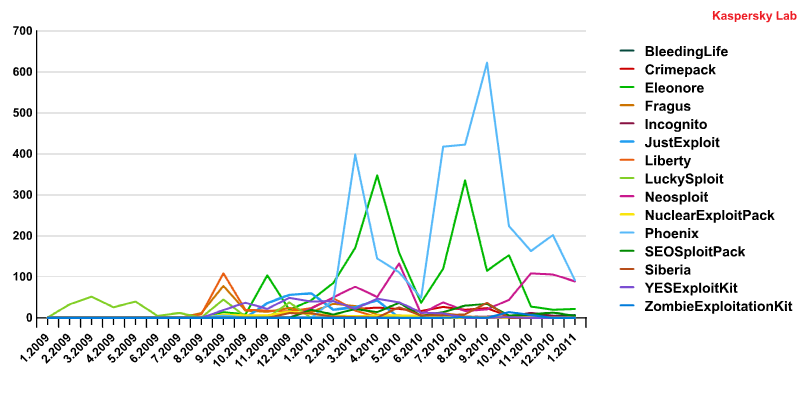
\includegraphics[scale=0.5]{Figures/kit.png}
\caption{L'évolution des kits d'exploitation.}
\label{fig :kit} 
\end{center}
\end{figure}
La figure~\ref{fig :kits} montre les vulnérabilités ciblées par ces kits d'exploitation :
\begin{figure}[H]
\begin{center}
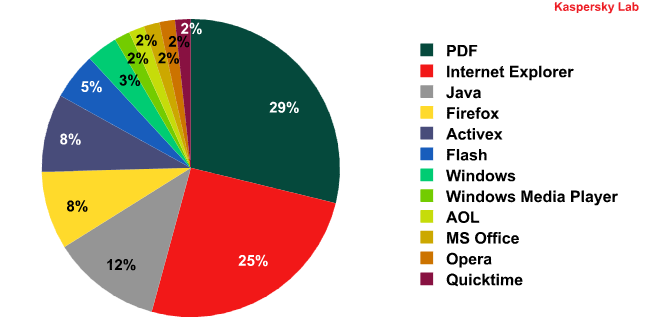
\includegraphics[scale=0.5]{Figures/kits.png}
\caption{Les vulnérabilités ciblées par les kits d'exploitation.}
\label{fig :kits} 
\end{center}
\end{figure}
Les vulnérabilités d’Internet Explorer, PDF et Java représentent 66\% des vecteurs d'attaque utilisés par les kits d'exploitation les plus répandus.
\subsection{ Les cycles de vie d'un malware}
Si on ignore la phase de conception et de test, par le créateur du malware,trois phases dans la vie d'un malware peuvent être identifiées. Leurs durées de vie respectives peuvent être plus ou moins longues, selon le type de malware et l'effet recherché.
\subsubsection{La phase d'infection}
Durant cette phase, le malware va se propager dans l'environnement informatique cible. Cela peut se produire de deux manières :
\begin{itemize}
\item Passivement : le malware est copie sur un support (disquette, CDROM , clef USB, site de téléchargement, forum de discussion... ) et transmis. Les victimes peuvent alors le copier dans leur propre environnement, avant de l'exécuter. 
\item Activement : l'utilisateur exécute le malware (cas de la première infection dans le système, appelée primo-infection) ou un fichier déjà contaminé lors d'une infection antérieure (primo-infection ou non).
\end{itemize}

\subsubsection{La phase d'incubation}
Cette phase constitue la plus grande partie de la vie d'un malware. La mission principale de cette phase est d'assurer la survie du malware, à travers toutes ses copies dans l'environnement cible. Il s'agit de limiter, voire  d'empêcher, sa détection:
\begin{itemize}
\item soit par l'utilisateur : en particulier, la phase de conception veillera tout particulièrement a éviter les erreurs d'exécution qui pourraient alerter l'utilisateur 
\item soit par l'antivirus : dans cette optique, le malware va développer plusieurs techniques qui vont lui permettre de se dérober à la surveillance antivirale.
\end{itemize}

\subsubsection{La phase de maladie}
Lors de cette phase, la charge finale est activée. Son mode de déclenchement peut dépendre de nombreux facteurs et sera fonction de l'endroit, dans le code, où la routine offensive sera placée :
\begin{itemize}
\item En tête de code, la charge finale sera systématiquement exécutée, avant
toute infection. Ce cas est rare, il a pour conséquence de limiter généralement la phase de survie du malware.
\item En fin de code, elle n'aura lieu qu'après les processus d'infection ;
\item Au milieu du code, en particulier si elle est conditionnée par la réussite
ou non de l'infection. 
\end{itemize}


\subsection{Les principales sources d'infection}
La plupart des sources d'infection sont les suivantes :\\


\begin{itemize}
\item \textbf{Internet :}Le réseau d'information global est la principale source de propagation de tout type de malware. En règle générale les virus et autres programmes malveillants sont situés sur des sites Web, déguisés sous forme de logiciels libres et utiles\\


\item \textbf{Le courrier électronique :}Les mails reçus par l'utilisateur stockés dans les bases de messagerie, peuvent aussi bien contenir des virus. Le malware peut être soit en pièce jointe ou être présent dans le corps d'un message. les données seront infectés, soit lors de l'ouverture du message ou lors de la sauvegarde sur un disque. Le courrier peut aussi être la source de deux autres menaces : le spam et le phishing. Si le spam causes principalement une perte de temps, le but du phishing est de récuperer la confidentialité des informations (par exemple numéro de carte de crédit)\\


\item \textbf{Vulnérabilités de logiciels :} Les vulnérabilités accordent aux hackers l'accès à distance, et donc aux données personnelles, aux ressources réseau via le LAN/Ethernet, et d'autres sources d'information\\


\item \textbf{Support amovible :} les disques amovibles sont largement utilisés pour transférer les informations, tel que les flash disk et les disques durs. Lors de l'ouverture d'un fichier enregistré sur un disque amovible, il peut endommager les données sur le système par un virus, et le diffuser sur d'autres lecteurs. 
\end{itemize}
\subsection{L'évolution des malwares}
\subsubsection{Tableau historique des malwares}
Le tableau \ref{malware} donne une liste des malwares les plus connus.
\begin{table}[H]
\begin{tabular}{|p{1.5cm}|p{2cm}|p{2cm}|p{9cm}|}
\hline \textbf{Date} &  \textbf{Nom} & \textbf{Type} & \textbf{Effets} \\
\hline 1986 & Brian & Virus & Infection du système de démarrage de la disquette et corruption des données de la disquette \\
\hline 1987 & Jerusalem & Virus & Infection et destruction de fichiers .exe et .com, résidant en mémoire\\
\hline 1988 & Morris Worm & Ver & Premier ver écrit pour Internet, infectant les ressources machines de l'utilisateur \\
\hline 1991 & Michelangelo & Bombe logique & Ecrasement des 256 premiers secteurs du disque dur le 6 mars 1991 \\
\hline 1999 & Melissa & Macro-virus & Via un fichier Word contaminé, la machine envoie par courrier électronique aux 50 premières adresses électroniques trouvées le fichier infecté\\
\hline 2000 & I love you & ver & Envoi massif du ver à tous les contacts Outlook, infection et corruption de fichiers et de bases de registres \\
\hline 2001 & Naked & Virus & Animation en Flash, présentant une femme nue, se diffusant à l'ensemble du carnet d'adresse et supprimant les répertoires Windows et systèmes \\
\hline 2002 & BugBear & Ver avec keylogger intégré & Installation d'un logiciel espion et envoie des enregistrements de frappes de clavier sur un serveur distant \\
\hline
\end{tabular}
%\caption{Tableau historique des malwares part 1}
\label{malware}
\end{table}
\begin{table}[H]
\begin{tabular}{|p{1.5cm}|p{2cm}|p{2cm}|p{9cm}|}
\hline \textbf{Date} &  \textbf{Nom} & \textbf{Type} & \textbf{Effets} \\
\hline 2003& Blaster & ver & Il fut aperçu pour la première fois dans la nature le 11 août. Sa vitesse de propagation augmenta exponentiellement jusqu'à atteindre un pic le 13 août. Le but de ce ver était de lancer une attaque en déni de service de type SYN flood. Pour se propager, le ver utilisait une vulnérabilité de type dépassement de tampon dans le service DCOM RPC, affectant le système d'exploitation dans son intégralité \\
\hline 2004 & Sasser & ver & il profite d'une vulnérabilité LSASS de Microsoft Windows pour télécharger sur la machine infectée un fichier nommé avserve.exe dans le répertoire Windows via FTP et le port TCP 5554 et lance son exécution à distance sans aucune intervention de l'utilisateur\\
\hline 2005 & GPCode  & Ransomware & Chiffrait les fichier et proposait à l'utilisateur de déchiffrer les fichiers en échange de 300\$\\
\hline 2006 & Nyxem & Ver avec bombe logique & Mass mailer qui supprimait les documents  Office, modifiant les paramètres systèmes, désactivant les antivirus, prévu pour s'exécuter le 3 février \\
\hline 2007 & Storm & Trojan & Dissimulé dans une pièce jointe, infection de la machine et transformation en zombie \\
\hline 2008 & Conficker& Ver & Ce ver exploite une vulnérabilité du Windows Server Service utilisé par Windows 2000, Windows XP, Windows Vista, Windows 7, Windows Server 2003 et Windows Server 2008\\
\hline 2009 & Psyb0t & Virus & Infection des routeurs DSL pouvant être manipulés sans mot de passe en raison d'un firmware trop vieux et transformation en zombie \\
\hline 2010 & Stuxnet & Ver & Stuxnet est un ver informatique supposé développé conjointement par les États-Unis et Israël pour s'attaquer à des systèmes iraniens. Spécifique au système Windows. La complexité du ver est très inhabituelle pour un malware. Il a été décrit par différents experts comme cyber arme, conçue pour attaquer une cible industrielle déterminée. Il s'agirait d'une première dans l'histoire. \\
\hline 2010 & Zeus/Zitmo & Trojan & interceptait les informations bancaires, découvert en 2007 mais une nouvelle variante voit le jour en 2010 en s'attaquant aux terminaux mobiles ainsi qu'aux consoles de jeux vidéo \\
\hline 2011 & DuQu & virus & Une vulnérabilité de Windows a été utilisée par des pirates pour mettre au point le virus DuQu, repéré le mois dernier. De façon classique, ce virus se transmet par courrier électronique dans un document Word infecté. Une fois l'ordinateur contaminé, les pirates peuvent prendre le contrôle de la machine à distance. Il aurait été créé par le même groupe à l'origine de Stuxnet\\
\hline
\end{tabular}
%\caption{Tableau historique des malwares}
\label{malware}
\end{table}
\begin{table}[H]
\begin{tabular}{|p{1.5cm}|p{2cm}|p{2cm}|p{9cm}|}
\hline \textbf{Date} &  \textbf{Nom} & \textbf{Type} & \textbf{Effets} \\
\hline 2012 & Flame & Virus & Considéré comme le descendant plus perfectionné que Stuxnet, il vise également les systèmes industriels sensibles, intercepte les données et exploite les vulnérabilités des machines Windows\\

\hline
\end{tabular}
\caption{Tableau historique des malwares}
\label{malware}
\end{table}

La figure \ref{fig :mal} montre que le nombre de malwares, entre 2005 et 2014, est dans une augmentation continue. \begin{figure}[H]
\begin{center}
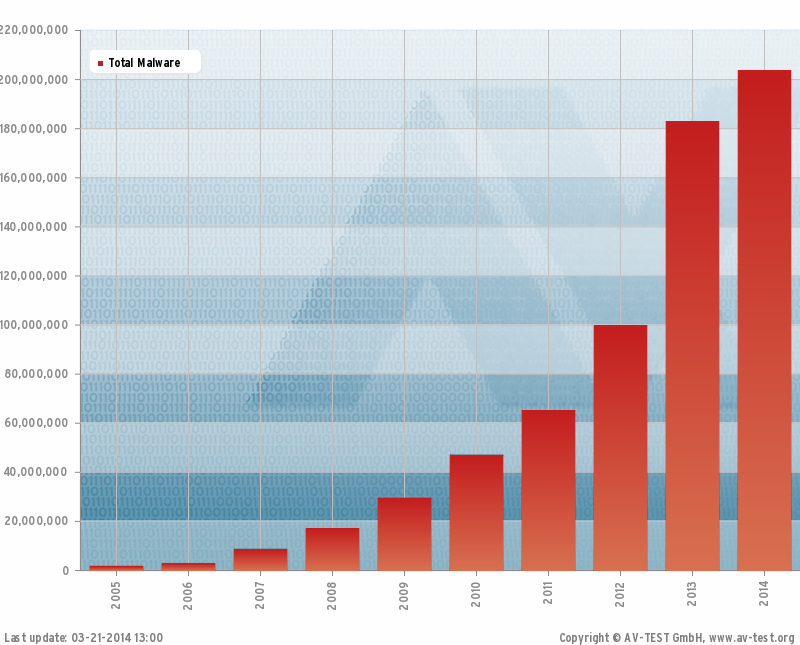
\includegraphics[scale=0.4]{Figures/mal.PNG}
\caption{nombre de malwares les dix dernières années}
\label{fig :mal} 
\end{center}
\end{figure}
\subsubsection{Evolution des malwares sur mobiles} 
Le nombre de malwares sur mobiles conçues pour des attaques de phishing, le vol de coordonnées de carte bancaire et d’argent sur les comptes en banque, a quasiment été multiplié par 20.\\

les mails sont aussi une source pour infecter les terminaux mobiles. les postes infectés forcent aussi l'utilisateur a télécharger et installer une application mobile malveillante sur son terminal. pour effectuer une fraude bancaire, la quasi totalité des banques envoient un code de sécurité par SMS à l'utilisateur. Le malware sur mobile a pour objectif d'intercepter et transférer ce code au cybercriminel, autrement il ne pourrait pas effectuer des virements bancaires à l'aide des identifiants de la victime. cette technique s'appelle "MITMO" : Malware In The MObile.\\


Les chevaux de Troie bancaires sont de loin les plus dangereux. Entre janvier et décembre 2013, leur nombre s’est multiplié. Kaspersky Lab dénombrait 67 chevaux de Troie bancaires connus début 2013, et à la fin de cette année-là, la base de données de Kaspersky Lab contenait déjà 1 321 variantes.\\


Les cybercriminels recourent de plus en plus à la technique d'obfuscation , qui consiste à rendre délibérément le code malveillant très complexe et donc plus difficile à analyser. Une solution antivirus mettra alors plus de temps à neutraliser le code laissant assez de temps aux cybercriminels pour arriver à leurs fins.\\


Parmi les méthodes pour infecter un mobile, on compte désormais la contamination via des sites légitimes compromis. La propagation du malware se fait par l'intermédiaire d’\textbf{app stores}  alternatifs et de bots (ces derniers s'autopropagent généralement par l'envoi des sms, contenant un lien malveillant, aux destinataires qui figurent dans le répertoire de la victime).\\

\subsubsection{2013 en chiffres}
Si l’on regarde 2013 de plus prêt, il est possible de constater l’énorme augmentation qu’ont connue les malwares mobiles. Néanmoins, bien que les malwares aient réussi à atteindre des sommets.
\begin{itemize}
\item En 2013, 3 905 502 paquets d’installations ont été utilisés par les cybercriminels pour distribuer les malwares mobiles
\item  les terminaux Android sont la cible priviligiée voire unique des malwares pour mobiles. Selon le rapport annuel 2014 de Cisco sur la sécurité ~\cite{cisco}, ces logiciels malveillants ciblent à 98\% les appareils Android. Sur cette plateforme, le malware mobile le plus répandu, à 43,8 pour cent, est \textbf{\textit{Andr/Qdplugin}} ~\cite{cisco}. voire figure ~\ref{fig :mobile}
\begin{figure}[H]
\begin{center}
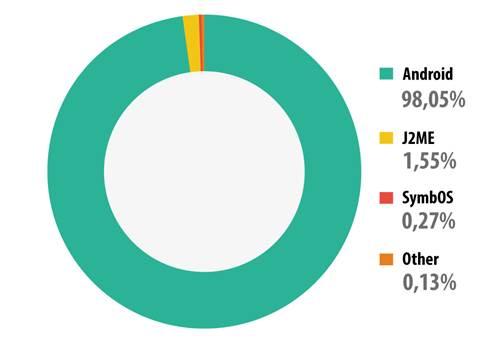
\includegraphics[scale=0.7]{Figures/mobile.jpg}
\caption{les plateformes ciblés par des malwares mobiles}
\label{fig :mobile} 
\end{center}
\end{figure}

\item La majorité des malwares mobiles(figure ~\ref{fig :mobile2}) est toujours spécialisée en vols d’argent mineurs grâce à des appels et à des messages vers des numéros surtaxés. Cependant, au cours de l’année, le nombre de modifications de malwares mobiles conçues pour le phishing, le vol d’informations de cartes bancaires ou d’argent a été multiplié par 19,7.
\begin{figure}[H]
\begin{center}
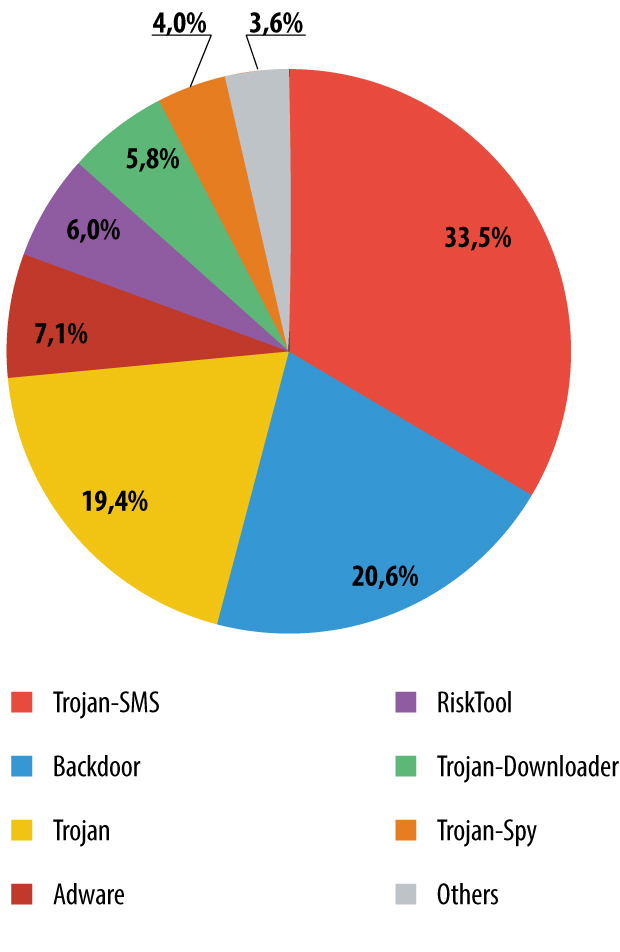
\includegraphics[scale=0.36]{Figures/mobile2.jpg}
\caption{Catégorie des malwares mobiles}
\label{fig :mobile2} 
\end{center}
\end{figure}

\end{itemize}
\subsubsection{Les malwares sur la plateforme GNU Linux}    


Le système d'exploitation Linux, au même titre que les systèmes d'exploitation Unix et apparentés, est généralement assez bien protégé contre les malwares. Cependant, certains programmes malveillants peuvent potentiellement endommager des systèmes GNU Linux non sécurisés.\\


Comme les autres systèmes Unix, Linux implémente un environnement multi-utilisateur, dans lequel les utilisateurs possèdent des droits spécifiques correspondant à leur besoin. Il existe ainsi un système de contrôle d'accès visant à interdire à un utilisateur de lire ou de modifier un fichier. Ainsi, les malwares ont typiquement moins de capacités à altérer et à infecter un système fonctionnant sous Linux que sous DOS ou encore les systèmes Microsoft Windows ayant toujours des systèmes de fichiers en FAT32 (le système de fichier NTFS a le même type de protection que les fichiers UNIX, les systèmes Microsoft Windows à base NT isolent également les comptes entre eux). C'est pourquoi, aucun des malwares écrits pour Linux, n'a pu se propager avec succès. En outre, les vulnérabilités qui sont exploitées par les malwares sont corrigées en quelques jours par les mises à jour du noyau Linux et des logiciels composant le système.\\


Des scanners du malwares sont disponibles pour des systèmes Linux afin de surveiller l'activité des malwares actifs sur Windows. Ils sont principalement utilisés sur des serveurs mandataires ou des serveurs de courrier électronique, qui ont pour client des systèmes Microsoft Windows.\\
\newpage
\textbf{\textit{Opération windigo :}}\\


Windigo est un malware qui prend la forme d’un cheval de Troie et qui se sert des serveurs Unix/Linux comme plateforme de diffusion de Spams. Différent pays sont touchés comme les USA, l'Allemagne, la France, L'Italie, la Grande Bretagne, les Pays-Bas, la Russie, l'Ukraine, le Mexique ou encore le Canada~\cite{windigo}.\\

Plus de 25000 serveurs ont été infectés par ce malware ces 2 dernières années, et plus de 10000 le sont toujours aujourd'hui. Ces serveurs sont principalement compromis par la vulnérabilité "Linux/Ebury". Le groupe à l'origine de la vulnérabilité "Linux/Ebury" est également l'auteur des vulnérabilités "Linux/Cdorked", "Perl/Calfbot" et "Win32/Glupteba.M".\\ 


Windigo s'appuie sur trois composants :
\begin{itemize}
\item \textbf{Linux/Ebury : }Backdoor OpenSSH pour garder un contrôle du serveur et pour voler les identifiants
\item \textbf{Linux/Cdorked : }Backdoor HTTP pour la redirection du trafic, ainsi qu’un serveur DNS modifié connu sous le nom de Linux/Onimiki
\item \textbf{Perl/Calfbot : }Script PERL pour générer du spam.

\end{itemize}
Les serveurs infectés redirigent plus d'un demi-million de visiteurs vers du contenu malicieux chaque jour. Ces serveurs donnent accès à une grande capacité de bande passante, de stockage, de puissance de calcul et de mémoire. Les attaquants sont capables d'envoyer plus de 35000000 pourriels par jours. Il est intéressant de noter que l'installation est faite de manière manuelle par les auteurs du malware.\\

Windigo affecte aussi bien les serveurs que les PC. Les systèmes d'exploitation affectés sont Linux, FreeBSD, OpenBSD, OS X, et même Microsoft Windows (avec Perl tournant sous Cygwin). Les serveurs cPanel et kernel.org font partie de la liste des victimes de ce malware. Il agit de différentes manières en fonction des systèmes :
\begin{itemize}

\item Sous Microsoft Windows il installe un kit d’exploitation
\item Sous MAC OS, il affiche des publicités pour des sites de rencontre
\item Sous IOS les utilisateurs sont redirigés vers des sites à contenu pornographique.

\end{itemize}
En cas d'infection, un formatage et une réinstallation complète du système sont nécessaires. la commande suivante dans un terminal permet de savoir si le système est infecté ou non :\\
\begin{lstlisting}
$ ssh -G 2>&1 | grep -e illegal -e unknown > /dev/null && echo "System clean"
 || echo "System infected"
\end{lstlisting}
\subsubsection{Les malwares sur la plateforme Mac OS X}
Nombreux sont ceux à croire que la plateforme Mac OS X de Apple est plus sécurisée que Microsoft Windows. Certains pensent que son mode UNIX pour la gestion des privilèges et des permissions lui confère une sécurité plus solide que Microsoft Windows, et sa gamme de matériel plus limitée implique moins de code et donc moins d'exposition aux vulnérabilités liées au code.\\


Pourtant, comme les Macs sont moins répandus en milieu professionnel, ils constituent une cible réduite pour les 
cybercriminels. Ceci explique que le problème des malwares sur Macs ne représente qu'une infime partie de ce que l'on peut voir sur les plateformes Microsoft Windows. Cependant, de nouveaux malwares continuent sans cesse d'émerger. Et même si
la zone d'attaques ne présente pas autant de possibilités d'infection et de propagation, les utilisateurs de Mac sont toujours vulnérables aux escroqueries et aux arnaques utilisées pour les piéger et les inciter à installer des logiciels suspects visant à accéder à leurs systèmes et à leurs données à distance.\\


Par exemple, 2010 a vu une nouvelle version du cheval de Troie OSX/Pinhead, qui se présente comme une copie de l'application iPhoto comprise avec tous les nouveaux Mac. Si l'utilisateur dupé installe le logiciel, il ouvre une porte dérobée qui donne aux pirates un plein accès au système compromis. Plus tard dans l'année, c'était au tour du cheval de Troie Boonana de viser les utilisateurs de Mac, Microsoft Windows et même GNU Linux. Il s'est propagé via des liens spammés sur Facebook et a utilisé des arnaques  classiques d'ingénierie sociale pour piéger ses victimes et leur faire installer une application Java, qui télécharge et exécute une autre série d'applications malveillantes.\\


En 2011, l'émergence des malwares Mac a attiré beaucoup d'attention. Il est évident que le problème des malwares Windows est
bien supérieur à la menace sur Mac, mais les évènements de 2011 ont rappelé aux utilisateurs Mac qu'ils devaient être
prudents. Les cybercriminels utilisent désormais les mêmes techniques sur Mac que sur PC, à savoir l'infection par les faux antivirus tels que MacDefender, Mac Security, MacProtector et MacGuard, qui sont tous apparus dans le courant de l'année.\\

Le système d'exploitation Mac OS X 10.7 d'Apple, surnommé Lion, prétend protéger l'utilisateur contre les malwares. Cependant, il ne détecte qu'un nombre limité de téléchargements malveillants issus de 10 différents types de malwares
Mac.\\


Bien que cette année la plate-forme Mac OS X n'ait pas subi d'attaque égalant l'étendue mondiale de Flashback en 2012, les attaques ont continué à évoluer en 2013, sous des formes diverses : chevaux de Troie, attaques contre les vulnérabilités de Java et les formats des documents Word, plug-ins agressifs, JavaScript malveillant et malwares conçus pour passer outre la protection Apple Gatekeeper grâce à une fausse identité Apple Developer.
\begin{figure}[H]
\begin{center}
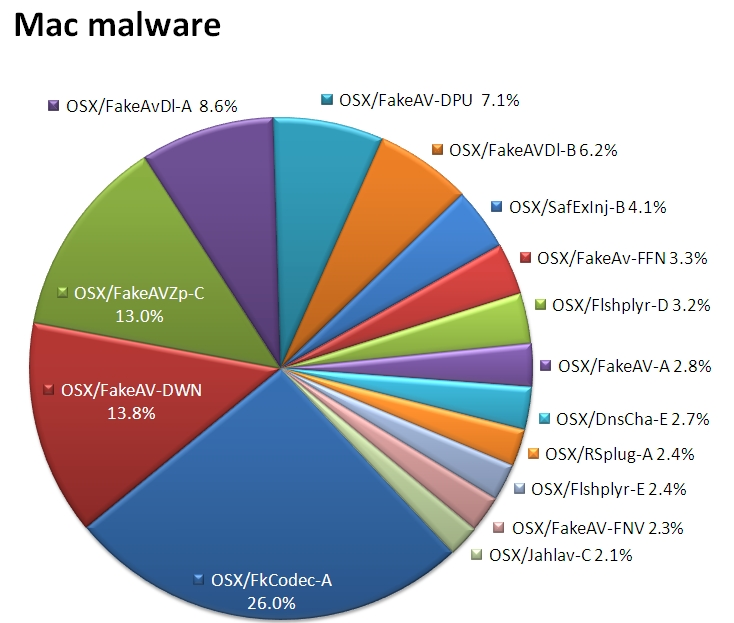
\includegraphics[scale=0.45]{Figures/mac.jpg}
\caption{Les malwares sous la plate-forme MAC OS X.}
\label{fig :kit} 
\end{center}
\end{figure}
\subsubsection{Les malwares multi-plateformes}
Récemment, les attaques contre les Mac, Facebook, Apple et Microsoft ont rappelé que les cybercriminels n'avaient pas que Microsoft Windows dans leurs lignes de mire. Et le fait de cibler deux voire plusieurs plateformes à la fois, comme le font déjà les adwares et les spams, devient de plus en plus fréquent pour les malware. En utilisant des langages de programmation multi-plateformes comme Java, les cybercriminels mettent en place des logiciels malveillants qui, en compromettant un site web, peuvent percevoir le système d'exploitation qu'utilise le visiteur. Ils y déposent un malware, affichent des publicités, redirigent l'internaute vers un site web frauduleux, tentant de générer de l'argent en s'adaptant à l'appareil servant à la connexion, quel qu'il soit.\\

Les malwares multi-plateformes, générés par la popularité des applications multi-plateformes ciblent généralement les macro des suites bureautiques, en particulier celles qui autorisent l'exécution de scripts comme ActiveX, mais cela peut se faire par l'ajout de plugins ou d'extensions provenant de sources non fiables. Cela est vrai aussi pour les navigateurs web.

\textbf{\textit{Exemples : }}\\
\begin{itemize}
\item Un botnet java multi-plateforme est utilisé dans des attaques DDOS. L'application Java malveillante peut être exécutée sur des machines Microsoft Windows, OS X et GNU Linux. L'éditeur de solutions de sécurité Kaspersky avertit sur son blog d'un nouveau malware utilisant une faille de la machine virtuelle Java. Même si la brèche a déjà été colmatée, nombreux sont les ordinateurs à posséder une ancienne mouture, ce qui rend la menace potentiellement sérieuse. Ce n'est pas la première fois qu'un botnet infecte les trois systèmes d'exploitation de bureau les plus populaires. Un côté multiplateforme que lui confère à chaque fois Java.\\


\item L'exemple le plus flagrant de malware multiplateforme est Zeus et sa version mobile Zeus-in-the-Mobile (ZitMo) qui avaient pour but de voler des données bancaires.\\
Zeus utilise un procédé assez simple. Le cheval de Troie commence par compromettre un ordinateur Microsoft Windows et attend que l'utilisateur ouvre son navigateur et accède à ses comptes en ligne. Ensuite, il ajoute des champs additionnels à la page Web de la banque, où il invite les utilisateurs à renseigner leurs numéro de téléphone ainsi que leurs modèle de téléphone mobile pour des soi-disant renouvellements de certificat. Par conséquent, les propriétaires du Zeus obtiennent toutes les informations qui ont été rentrées sur la page modifiée, y compris toutes les informations bancaires requises en ligne. Après cela, un SMS est envoyé au numéro de téléphone qu'avez renseigné : celui-ci contient un lien vers un certificat qui n'existe pas et qui est en fait le cheval de Troie, ZitMo. Une fois le smartphone infecté, le malware mobile commence à intercepter les codes d'autorisation et les notifications de mouvement sur le compte qui sont envoyés par SMS par la banque. Ainsi, sans que vous le sachiez, le cybercriminel pourra travailler à distance sur le compte bancaire de la victime en utilisant des données volées.
\end{itemize}

\section{Les Antivirus}

\subsection{Définition}
Il s'agit d'un logiciel capable de détecter et de détruire les virus contenus sur un disque. Le logiciel a pour charge de surveiller la présence de virus et éventuellement de nettoyer, supprimer ou mettre en quarantaine le ou les fichiers infectés. Ils surveillent tous les espaces dans lesquels un virus peut se loger, c'est à dire la mémoire et les unités de stockage qui peuvent être locales ou sur le réseau~\cite{anti}.
\subsection{Fonctionnement des Antivirus}
les antivirus fonctionnent à quelques rares exceptions près - selon deux modes : ~\cite{anti}
\subsubsection{Mode statique :} 
L'antivirus n'est alors actif que par une action volontaire
de l'utilisateur (déclenchement manuel ou pré-programmé), il est donc le plus souvent inactif et aucune détection n'est possible. C'est le mode le plus adapté aux machines de faible puissance. La technique de surveillance de comportement n'est pas disponible dans ce mode.\\
Notre antivirus qu'on va déployer, il sera en mode statique.
\subsubsection{Mode dynamique :}
l'antivirus est, en fait, résident et surveille en permanence l'activité du système d'exploitation, du réseau et surtout de l'utilisateur. II prend la main avant toute action et tente de déterminer si un risque viral existe, lié à cette action. Ce mode est gourmand en ressources et nécessite des machines relativement puissantes, pour ne pas être handicapant et pousser l'utilisateur (cas trop souvent rencontré) a désactiver ce mode au profit du précédent.
\subsection{Les techniques antivirales}
Les antivirus modernes, pour les plus efficaces, conjuguent plusieurs techniques afin de réduire le risque de fausses alarmes et de non-détection, au minimum. Elles peuvent être classees en deux groupes : les techniques statiques et les techniques dynamiques~\cite{anti}.
\subsubsection{Recherche de signatures}
Cette technique consiste a rechercher une suite d'octets, caractéristique d'un malware donné. Cette suite est analogue à l'empreinte digitale d'une personne. Utilisée comme signature, elle doit posséder deux propriétés importantes ~\cite{anti} :
\begin{itemize}
\item Elle doit être \textit{discriminante}. Cela signifie que la signature doit identifier spécifiquement le malware
\item Elle doit être \textit{non incriminante}. Autrement dit, elle ne doit théoriquement
pas incriminer un autre malware, ou un programme sain. Elle doit donc posséder une taille et des caractéristiques suffisamment pertinentes pour ne pas provoquer de faux positifs.
\end{itemize}

En général, plus la séquence utilisée pour définir la signature est longue, plus cette signature réalisera ces deux propriétés.\\


Cette signature peut être :
\begin{itemize}
\item soit une séquence d'instructions;
\item soit un message affiché par le malware;
\item soit tout simplement la signature que le malware lui-même utilise pour éviter la surinfection d'un exécutable.
\end{itemize}


La base de signatures comporte, pour chaque malware qui s'y trouve recensé :
\begin{itemize}
\item La signature proprement dite;
\item l'endroit où la chercher (en-tête de Inexécutable, début ou fin du code... ).
plutot que de rechercher la séquence d'octets qui la définit dans tout l'exécutable. l'antivirus se limite a une zone spécifique de cet exécutable, cela permet d'accélérer la recherche;
\item le mode de recherche : recherche simple de la signature, décompression du code, déchiffrement ...\\
\item le nom du malware : quand l'antivirus identifie une souche virale, il informe l'utilisateur en utilisant le nom du malware comme : duqu, stuxnet, conficker, blaster, sasser, zeus, ...
\end{itemize}


Si la détection par signatures peut se révéler très efficace, elle se limite aux
malwares connus et analysés. Le problème avec cette technique est qu'elle est facilement
contournable. Un simple changement de compilateur suffit à leurrer la plupart des antivirus. Elle ne permet de gérer ni les virus polymorphes, ni certains virus chiffrés, et encore moins les malwares inconnus. Le taux de faux positifs est faible bien que l'identification correcte laisse quelquefois à désirer (problème de fausse incrimination).\\

Le principal inconvénient  de ce mode de détection est la nécessité de maintenir la base de signatures virales avec les contraintes que cela comporte :taille de la base, stockage sécurisé (des sites d'antivirus contenant les bases de signatures de leurs produits sont quelquefois attaqués), la distribution sécurisée, la mise à jour plus ou moins régulière et effective par l'utilisateur, souvent négligent. A noter que la mise à
jour de ces bases permet la détection de nouveaux malwares, mais aussi, dans certains cas, d'améliorer la détection des malwares précédemment repérés (par d'autres techniques) en diminuant, par exemple, les ressources machine nécessaires.\\
\subsubsection{Analyse spectrale}
L'analyse spectrale repose sur le postulat que tout code généré automatiquement contiendra des signes révélateurs du compilateur utilisé. De même, on part du principe qu'il est impossible de retrouver dans un vrai programme exécutable compilé certaines séquences de code. L'analyse spectrale vise donc elle aussi à repérer les virus polymorphes ou inconnus. Lorsqu'un virus polymorphe chiffre son code, la séquence en résultant contient certaines associations d'instructions que l'on ne trouverait pas dans un vrai programme. C'est ce que l'analyse spectrale tente de détecter. Par exemple, si dans un programme exécutable, l'antivirus trouve une instruction de lecture d'un octet au delà de la taille limite de la mémoire, on sera
probablement en présence de code chiffré, packé ou polymorphe~\cite{anti}.\\
\subsubsection{Contrôle d'intégrité}
Puisque les virus modifient les programmes qu'ils infectent, certains antivirus utilisent un contrôleur d'intégrité pour vérifier si les fichiers de la machine ont été modifiés. Ainsi, une base de données est construite, qui contient des détails sur les fichiers exécutables du système, comme leur taille ou leur date de modification, et éventuellement un condensé cryptographique (checksum).. Dès lors, si une de ces caractéristiques change pour un exécutable, l'antivirus s'en aperçoit~\cite{antiv}.

\subsubsection{La surveillance comportementale}
L'antivirus est résident en mémoire et tente d'identifier tout comportement suspect (la définition d'un tel comportement se faisant par rapport à une base de comportements viraux) et le bloquer si nécessaire.
Les actions suivantes peuvent être identifiées comme malveillantes : tentatives d'ouvertures en lecture/écriture de fichiers exécutables, écriture sur des secteurs systèmes (partition ou démarrage), tentative de mise en résident, etc.\\
Techniquement, l'antivirus agit par détournement d'interruptions (le plus souvent, les interruptions 13H et 21H) ou d'API.\\
Cette technique permet de détecter quelquefois des malwares inconnus (utilisant cependant des techniques connues) et de lutter avant l'infection. Toutefois, certaines techniques virales y échappent. De plus, l'antivirus doit être en mode dynamique, ce qui ralentit, quelquefois sensiblement, le système. Les faux positifs sont relativement nombreuses. Notons que l'analyse de l'antivirus permet de connaitre la base de comportements et tout le jeu du
programmeur du malware consistera à utiliser cette connaissance pour mieux contourner la protection~\cite{anti}.


\subsubsection{L'émulation de code}
Cette technique permet de disposer de la surveillance de comportement en mode statique, ce qui est assez utile car beaucoup d'utilisateurs impatients préfèrent ce mode pourtant dangereux. Lors du scan, le code étudié est chargé dans une zone memoire confinée, puis est émulé afin de détecter un comportement potentiellement viral. L'émulation de code est particulièrement
adaptée à la lutte contre les virus polymorphes. Cette technique souffre toutefois des mêmes limitations que son homologue dynamique~\cite{anti}.
\subsection{Eradication des malwares}
\subsubsection{Méthode d'éradication}
Une fois un malware détecté, il faut le supprimer. Mais il n'est pas toujours simple de supprimer un malware  sans endommager le programme original. En effet, certains programmes malicieux  détruisent une partie du programme sain lors de leur duplication. Il ne reste plus alors qu'à détruire purement et simplement le fichier infecté. Dans les autres cas, la suppression d'un malware n'est pas forcément évidente non plus. Il s'agit d'abord de découvrir très précisément où est localisé le malware dans le fichier, sachant qu'il peut être composé de plusieurs parties. Il faut ensuite supprimer ces octets infectés, et récupérer la partie du programme dont le malware avait pris la place, afin de la restaurer. Toutes ces manipulations nécessitent bien sûr une parfaite connaissance du malware et de son mode opératoire. C'est à cela que servent les fichiers de signatures des antivirus, régulièrement remis à jour. Il faut non seulement pouvoir détecter le virus, mais aussi savoir où il cache la portion de code dont il a pris la place~\cite{antiv}.
\subsubsection{Mise à jour des antivirus}
Cela pose donc la problématique de la mise à jour rapide des antivirus, et donc de la mise à disposition rapide des signatures de détection et méthodes de désinfection.\\


L'efficacité des solutions antivirus dépend des bases de données de définitions du malware. Ces bases sont dynamiques par nature étant donné la constante activité des auteurs des malwares. Par exemple, les analystes viraux de Kaspersky Lab détectent et ajoutent 100 nouvelles menaces quotidiennement à la base antivirus.\\


Les antivirus sont devenus de plus en plus sophistiqués au fil des années afin de contrer la complexité croissante des programmes malicieux. Des mécanismes de protection proactifs, heuristiques, conçus pour détecter les nouvelles menaces avant qu'elles n'apparaissent dans la nature offrent une première ligne de défense importante.\\


Néanmoins, une mise à jour régulière de la protection antivirus est plus importante que jamais étant donné la rapidité à laquelle les menaces actuelles sont capables de se propager. Les éditeurs d'antivirus ont réduit l'intervalle entre les mises à jour de signatures de trimestriellement à mensuellement et finalement à quotidiennement. Malgré toutes ces bonnes intentions, rien ne garantit que l'utilisateur final effectuera des mises à jour assez régulières. Ni qu'un virus à propagation rapide n'aura pas déjà infecté les machines avant la mise à disposition de mise à jour~\cite{antivirus}.
\section{Le besoin de l'analyse des malwares}
Tout comme l'écriture de code malveillant, il y a une myriade de raisons d'analyser les virus, les vers et les trojans. La raison principale derrière cela est qu'il n'y a aucun code source disponible pour de tels programmes. Le seul
moyen de comprendre ces programmes est de les analyser et déterminer leur fonctionnement interne. Une autre raison pourrait être que beaucoup de chercheurs aiment explorer les fonctionnements cachés d'un programme en l'examinant avec un désassembleur et un débogueur.\\


Il y a deux techniques majeures pour analyser ce code :\\

\begin{itemize}
\item \textbf{\textit{l'analyse statique : }}L'analyse statique de malwares consiste à explorer le contenu des fichiers suspects à l'aide de divers outils, dans le but d'extraire le maximum d'informations sans exécuter le code malveillant qu'ils pourraient contenir. A ce stade il s'agit uniquement d'observer le contenu "visible"\\
\item \textbf{\textit{l'analyse dynamique : }}Contrairement à l'analyse statiques, l'analyse dynamique consiste à exécuter réellement le code malveillant dans un environnement adéquat afin d'observer toutes ses actions et d'en déduire son comportement global. Ce type de méthode est parfois appelée analyse comportementale.\\

\end{itemize}


Ces deux techniques seront discutées dans le chapitre 5.
\section{Conclusion}
Tout au long de ce chapitre, une problématique majeure de la sécurité informatique a été abordée : les malwares.
Il a été constaté qu'il existait plusieurs types de malware, tel que les virus, les vers, les trojans ...\\


Les éditeurs d'antivirus ont donc de beaux jours devant eux, leur fond de commerce n'étant pas prêt de disparaître. Il leur faut néanmoins travailler d'arrache-pied pour trouver (ou améliorer) de nouvelles solutions pour combattre ce
fléau. Car, à chaque innovation des antivirus, les virus franchissent eux aussi un cap. Avec un avantage majeur à l'heure actuelle : il faut qu'ils soient découverts avant de pouvoir être combattus...\\


Si, aujourd'hui, Microsoft Windows est le système d'exploitation majoritairement touché, il est à craindre qu'avec l'explosion de GNU Linux et Apple Mac OS, et son arrivée imminente dans un plus grand nombre de foyers, fasse augmenter les attaques tournées vers ces systèmes. Surtout si des utilisateurs moins expérimentés viennent à l'utiliser. Il a cependant
une bonne marge d'avance, puisque le nombre de virus en activité sous Linux est dérisoire par rapport à ceux pour l'OS de Microsoft.\\


Dans le chapitre suivant on va parler sur les fichiers de format PE (Portable exécutable) 
de Microsoft Windows avec détailles parce que les antivirus doivent être capable de parser le format PE afin de pouvoir appliquer les différentes méthodes de détection (signature, émulation de code, ...). Aussi a connaissance du format PE est importante pour l'analyste afin de mieux comprendre et analyser manuellement le malware.